% !Rnw weave = knitr

\documentclass{article}\usepackage[]{graphicx}\usepackage[]{color}
%% maxwidth is the original width if it is less than linewidth
%% otherwise use linewidth (to make sure the graphics do not exceed the margin)
\makeatletter
\def\maxwidth{ %
  \ifdim\Gin@nat@width>\linewidth
    \linewidth
  \else
    \Gin@nat@width
  \fi
}
\makeatother

\definecolor{fgcolor}{rgb}{0.345, 0.345, 0.345}
\newcommand{\hlnum}[1]{\textcolor[rgb]{0.686,0.059,0.569}{#1}}%
\newcommand{\hlstr}[1]{\textcolor[rgb]{0.192,0.494,0.8}{#1}}%
\newcommand{\hlcom}[1]{\textcolor[rgb]{0.678,0.584,0.686}{\textit{#1}}}%
\newcommand{\hlopt}[1]{\textcolor[rgb]{0,0,0}{#1}}%
\newcommand{\hlstd}[1]{\textcolor[rgb]{0.345,0.345,0.345}{#1}}%
\newcommand{\hlkwa}[1]{\textcolor[rgb]{0.161,0.373,0.58}{\textbf{#1}}}%
\newcommand{\hlkwb}[1]{\textcolor[rgb]{0.69,0.353,0.396}{#1}}%
\newcommand{\hlkwc}[1]{\textcolor[rgb]{0.333,0.667,0.333}{#1}}%
\newcommand{\hlkwd}[1]{\textcolor[rgb]{0.737,0.353,0.396}{\textbf{#1}}}%

\usepackage{framed}
\makeatletter
\newenvironment{kframe}{%
 \def\at@end@of@kframe{}%
 \ifinner\ifhmode%
  \def\at@end@of@kframe{\end{minipage}}%
  \begin{minipage}{\columnwidth}%
 \fi\fi%
 \def\FrameCommand##1{\hskip\@totalleftmargin \hskip-\fboxsep
 \colorbox{shadecolor}{##1}\hskip-\fboxsep
     % There is no \\@totalrightmargin, so:
     \hskip-\linewidth \hskip-\@totalleftmargin \hskip\columnwidth}%
 \MakeFramed {\advance\hsize-\width
   \@totalleftmargin\z@ \linewidth\hsize
   \@setminipage}}%
 {\par\unskip\endMakeFramed%
 \at@end@of@kframe}
\makeatother

\definecolor{shadecolor}{rgb}{.97, .97, .97}
\definecolor{messagecolor}{rgb}{0, 0, 0}
\definecolor{warningcolor}{rgb}{1, 0, 1}
\definecolor{errorcolor}{rgb}{1, 0, 0}
\newenvironment{knitrout}{}{} % an empty environment to be redefined in TeX

\usepackage{alltt}

\usepackage{url}
\usepackage{underscore}

\title{Functional analysis of gene lists}
\author{Ferran Brians\'o and Alex S\'anchez-Pla. \\ Statistics department. UB \\ \& Statistics and Bioinformatics Unit (UEB). VHIR.}

\bibliographystyle{plain}
\IfFileExists{upquote.sty}{\usepackage{upquote}}{}
\begin{document}

\maketitle
\tableofcontents









\section{Introduction}

This document provides information on how to extract subsets of genes from previously available gene lists by setting different filtering conditions such as the fold change, the p-value or the availability of \texttt{Entrez} identifier.

\subsection{From gene lists to Functional Analysis}

The main, but not the only, goal of creating a gene list is to use it as input for some type of functional analysis such as Enrichment Analyis (ORA) or Gene set Enrichment Analysis (GSEA).

Functional analysis can be made, on a first approach on
\begin{itemize}
\item A list of genes selected by being differentially expressed in a given experimental setting.
\item The whole list of genes -or even the whole expression matrix- that has been used in the analysis.
\end{itemize}

Most tools require that gene list consist of gene identifiers in some standard notation such as \texttt{Entrez}, \texttt{ENSEMBL} or other related to these.

These gene lists can be easily extracted from output tables provided by microarrays or RNA-seq data analysis tools.

The analysis below is applied on a set of three gene lists obtained from a breast cancer study, but it can be easily extended to more lists or other studies.

\subsection{Data Input Format for gene list selection}

In principle a filtering tool might read the file header and, once this is done, create an interactive dialog to query for the values that would be applied for subsetting the lists rows or columns.

In practice, and in our work environment most lists will be extracted from the standard output of our microarray analysis pipeline\footnote{In this point we assume that the user is familiarized with standard microarray analysis ``a la Bioconductor''. If this is not so the reader can browse through the slides and examples in \url{http://eib.stat.ub.edu/Omics+Data+Analysis}}. These files are generically described as "Expression_and_TopTables" because they consist of tables having:
\begin{enumerate}
\item The Gene Symbols and the Entrez Identifiers in the first two columns
\item The standard output of the limma software known as "topTable"
\item [optionally] the Expression values that have been used to compute the Toptable. \footnote{Although some type of analyses require only the gene identifiers other need also the expressions. For this reason these output files contain ``all that is needed'' for further analyses}.
\end{enumerate}

\begin{knitrout}
\definecolor{shadecolor}{rgb}{0.969, 0.969, 0.969}\color{fgcolor}\begin{kframe}
\begin{alltt}
\hlstd{x1}\hlkwb{<-} \hlstd{AvsB} \hlkwb{<-} \hlkwd{read.table}\hlstd{(}\hlkwd{file.path}\hlstd{(dataDir,} \hlstr{"ExpressAndTop_AvsB.csv2"}\hlstd{),} \hlkwc{head}\hlstd{=T,} \hlkwc{sep}\hlstd{=}\hlstr{";"}\hlstd{,} \hlkwc{dec}\hlstd{=}\hlstr{","}\hlstd{,} \hlkwc{row.names}\hlstd{=}\hlnum{1}\hlstd{)}
\hlstd{x2}\hlkwb{<-} \hlstd{AvsL} \hlkwb{<-} \hlkwd{read.table}\hlstd{(}\hlkwd{file.path}\hlstd{(dataDir,} \hlstr{"ExpressAndTop_AvsL.csv2"}\hlstd{),} \hlkwc{head}\hlstd{=T,} \hlkwc{sep}\hlstd{=}\hlstr{";"}\hlstd{,} \hlkwc{dec}\hlstd{=}\hlstr{","}\hlstd{,} \hlkwc{row.names}\hlstd{=}\hlnum{1}\hlstd{)}
\hlstd{x3}\hlkwb{<-} \hlstd{BvsL} \hlkwb{<-} \hlkwd{read.table}\hlstd{(}\hlkwd{file.path}\hlstd{(dataDir,} \hlstr{"ExpressAndTop_BvsL.csv2"}\hlstd{),} \hlkwc{head}\hlstd{=T,} \hlkwc{sep}\hlstd{=}\hlstr{";"}\hlstd{,} \hlkwc{dec}\hlstd{=}\hlstr{","}\hlstd{,} \hlkwc{row.names}\hlstd{=}\hlnum{1}\hlstd{)}

\hlkwd{dim}\hlstd{(x1);}
\end{alltt}
\begin{verbatim}
## [1] 6221   18
\end{verbatim}
\begin{alltt}
\hlkwd{cat}\hlstd{(}\hlstr{"\textbackslash{}nHeader of top Table for comparison AvsB\textbackslash{}n"}\hlstd{)}
\end{alltt}
\begin{verbatim}
## 
## Header of top Table for comparison AvsB
\end{verbatim}
\begin{alltt}
\hlkwd{cat}\hlstd{(}\hlstr{"--------------------------------------------\textbackslash{}n"}\hlstd{)}
\end{alltt}
\begin{verbatim}
## --------------------------------------------
\end{verbatim}
\begin{alltt}
\hlkwd{head}\hlstd{(x1[}\hlnum{1}\hlopt{:}\hlnum{10}\hlstd{,} \hlnum{1}\hlopt{:}\hlnum{8}\hlstd{])}
\end{alltt}
\begin{verbatim}
##             SymbolsA EntrezsA     logFC  AveExpr          t      P.Value
## 204667_at      FOXA1     3169 -3.038344 8.651157 -14.362164 5.741793e-11
## 215729_s_at    VGLL1    51442  3.452290 6.137595  12.814829 3.439769e-10
## 220192_x_at    SPDEF    25803 -3.016315 9.521883 -10.859194 4.337504e-09
## 214451_at     TFAP2B     7021 -5.665059 7.432823 -10.829548 4.519412e-09
## 217528_at      CLCA2     9635 -5.622086 6.763101  -9.666128 2.431610e-08
## 217284_x_at   SERHL2   253190 -4.313116 9.133307  -9.528373 2.996253e-08
##                adj.P.Val         B
## 204667_at   3.571969e-07 14.648730
## 215729_s_at 1.069940e-06 13.148992
## 220192_x_at 7.028816e-06 10.928314
## 214451_at   7.028816e-06 10.891489
## 217528_at   3.025409e-05  9.363419
## 217284_x_at 3.106615e-05  9.171294
\end{verbatim}
\begin{alltt}
\hlkwd{cat}\hlstd{(}\hlstr{"\textbackslash{}nHeader of top Table for comparison AvsL\textbackslash{}n"}\hlstd{)}
\end{alltt}
\begin{verbatim}
## 
## Header of top Table for comparison AvsL
\end{verbatim}
\begin{alltt}
\hlkwd{cat}\hlstd{(}\hlstr{"--------------------------------------------\textbackslash{}n"}\hlstd{)}
\end{alltt}
\begin{verbatim}
## --------------------------------------------
\end{verbatim}
\begin{alltt}
\hlkwd{dim}\hlstd{(x2);} \hlkwd{head}\hlstd{(x2[}\hlnum{1}\hlopt{:}\hlnum{10}\hlstd{,} \hlnum{1}\hlopt{:}\hlnum{8}\hlstd{])}
\end{alltt}
\begin{verbatim}
## [1] 6221   18
##             SymbolsA EntrezsA     logFC  AveExpr         t      P.Value
## 205009_at       TFF1     7031  4.735050 8.692478 10.564670 6.548729e-09
## 205862_at      GREB1     9687  3.958563 6.082835  9.983993 1.513906e-08
## 205225_at       ESR1     2099  3.964939 9.300546  9.849787 1.846739e-08
## 209443_at   SERPINA5     5104  2.198392 7.586226  8.531873 1.448630e-07
## 217528_at      CLCA2     9635 -4.429254 6.763101 -7.615275 6.877151e-07
## 205696_s_at    GFRA1     2674  2.333785 6.239876  7.600491 7.058428e-07
##                adj.P.Val         B
## 205009_at   3.829521e-05 10.133204
## 205862_at   3.829521e-05  9.434088
## 205225_at   3.829521e-05  9.266376
## 209443_at   2.252982e-04  7.488507
## 217528_at   7.318414e-04  6.101859
## 205696_s_at 7.318414e-04  6.078427
\end{verbatim}
\begin{alltt}
\hlkwd{cat}\hlstd{(}\hlstr{"\textbackslash{}nHeader of top Table for comparison BvsL\textbackslash{}n"}\hlstd{)}
\end{alltt}
\begin{verbatim}
## 
## Header of top Table for comparison BvsL
\end{verbatim}
\begin{alltt}
\hlkwd{cat}\hlstd{(}\hlstr{"--------------------------------------------\textbackslash{}n"}\hlstd{)}
\end{alltt}
\begin{verbatim}
## --------------------------------------------
\end{verbatim}
\begin{alltt}
\hlkwd{dim}\hlstd{(x3);} \hlkwd{head}\hlstd{(x3[}\hlnum{1}\hlopt{:}\hlnum{10}\hlstd{,} \hlnum{1}\hlopt{:}\hlnum{8}\hlstd{])}
\end{alltt}
\begin{verbatim}
## [1] 6221   18
##             SymbolsA EntrezsA     logFC   AveExpr          t      P.Value
## 204667_at      FOXA1     3169  2.961042  8.651157  13.996760 8.630583e-11
## 215729_s_at    VGLL1    51442 -3.744599  6.137595 -13.899875 9.630024e-11
## 205009_at       TFF1     7031  5.729322  8.692478  12.783054 3.575181e-10
## 205225_at       ESR1     2099  3.939276  9.300546   9.786035 2.030957e-08
## 205862_at      GREB1     9687  3.774303  6.082835   9.519268 3.038123e-08
## 218211_s_at     MLPH    79083  2.808408 10.932769   8.813968 9.162548e-08
##                adj.P.Val         B
## 204667_at   2.995419e-07 14.040383
## 215729_s_at 2.995419e-07 13.953517
## 205009_at   7.413733e-07 12.893342
## 205225_at   3.158646e-05  9.422443
## 205862_at   3.780032e-05  9.061947
## 218211_s_at 8.534352e-05  8.062668
\end{verbatim}
\end{kframe}
\end{knitrout}

\section{Input data preprocessing}

Sometimes lists may need some preprocessing (e.g. in this example the gene list has multiple transcripts per gene identifier that have to be unitized previous to the analysis).

We have prepared two functions that encapsulate some standard functionalities for gene list filtering.

\begin{knitrout}
\definecolor{shadecolor}{rgb}{0.969, 0.969, 0.969}\color{fgcolor}\begin{kframe}
\begin{alltt}
\hlkwd{source}\hlstd{(}\hlstr{"https://raw.githubusercontent.com/alexsanchezpla/scripts/master/usefulFunctions/genesFromTopTable.R"}\hlstd{)}
\hlkwd{source}\hlstd{(}\hlstr{"https://raw.githubusercontent.com/alexsanchezpla/scripts/master/usefulFunctions/extractInfoFromTopTable.R"}\hlstd{)}
\end{alltt}
\end{kframe}
\end{knitrout}


We can use the available functions to extract only the gene lists
\begin{knitrout}
\definecolor{shadecolor}{rgb}{0.969, 0.969, 0.969}\color{fgcolor}\begin{kframe}
\begin{alltt}
\hlstd{geneList1}  \hlkwb{<-} \hlkwd{genesFromTopTable} \hlstd{(x1,} \hlkwc{entrezOnly} \hlstd{=} \hlnum{TRUE}\hlstd{,} \hlkwc{uniqueIds}\hlstd{=}\hlnum{TRUE}\hlstd{,}
                                 \hlkwc{adjOrrawP} \hlstd{=} \hlstr{"adj"}\hlstd{,} \hlkwc{Pcutoff} \hlstd{=} \hlnum{0.1}\hlstd{,} \hlkwc{FCcutoff} \hlstd{=} \hlnum{.75}\hlstd{,}
                                 \hlkwc{id2Select} \hlstd{=} \hlstr{"SymbolsA"} \hlstd{,} \hlkwc{cols2Select} \hlstd{=}\hlnum{3}\hlstd{)}
\hlkwd{length}\hlstd{(geneList1)}
\end{alltt}
\begin{verbatim}
## [1] 874
\end{verbatim}
\begin{alltt}
\hlstd{geneList1Up}  \hlkwb{<-} \hlkwd{genesFromTopTable} \hlstd{(x1,} \hlkwc{entrezOnly} \hlstd{=} \hlnum{TRUE}\hlstd{,} \hlkwc{uniqueIds}\hlstd{=}\hlnum{TRUE}\hlstd{,}
                                 \hlkwc{adjOrrawP} \hlstd{=} \hlstr{"adj"}\hlstd{,} \hlkwc{Pcutoff} \hlstd{=} \hlnum{0.1}\hlstd{,} \hlkwc{FCcutoff} \hlstd{=} \hlnum{.75}\hlstd{,} \hlkwc{updown}\hlstd{=}\hlstr{"up"}\hlstd{,}
                                 \hlkwc{id2Select} \hlstd{=} \hlstr{"EntrezsA"} \hlstd{,} \hlkwc{cols2Select} \hlstd{=}\hlnum{3}\hlstd{)}
\hlkwd{length}\hlstd{(geneList1Up)}
\end{alltt}
\begin{verbatim}
## [1] 534
\end{verbatim}
\begin{alltt}
\hlstd{geneList1Down}  \hlkwb{<-} \hlkwd{genesFromTopTable} \hlstd{(x1,} \hlkwc{entrezOnly} \hlstd{=} \hlnum{TRUE}\hlstd{,} \hlkwc{uniqueIds}\hlstd{=}\hlnum{TRUE}\hlstd{,}
                                 \hlkwc{adjOrrawP} \hlstd{=} \hlstr{"adj"}\hlstd{,} \hlkwc{Pcutoff} \hlstd{=} \hlnum{0.1}\hlstd{,} \hlkwc{FCcutoff} \hlstd{=} \hlnum{.75}\hlstd{,} \hlkwc{updown}\hlstd{=}\hlstr{"down"}\hlstd{,}
                                 \hlkwc{id2Select} \hlstd{=} \hlstr{"EntrezsA"} \hlstd{,} \hlkwc{cols2Select} \hlstd{=}\hlnum{3}\hlstd{)}
\hlkwd{length}\hlstd{(geneList1Down)}
\end{alltt}
\begin{verbatim}
## [1] 340
\end{verbatim}
\begin{alltt}
\hlstd{geneList2} \hlkwb{<-} \hlkwd{genesFromTopTable} \hlstd{(x2,} \hlkwc{entrezOnly} \hlstd{=} \hlnum{TRUE}\hlstd{,} \hlkwc{uniqueIds}\hlstd{=}\hlnum{TRUE}\hlstd{,}
                                 \hlkwc{adjOrrawP} \hlstd{=} \hlstr{"adj"}\hlstd{,} \hlkwc{Pcutoff} \hlstd{=} \hlnum{0.1}\hlstd{,} \hlkwc{FCcutoff} \hlstd{=} \hlnum{.75}\hlstd{,}
                                 \hlkwc{id2Select} \hlstd{=} \hlstr{"EntrezsA"} \hlstd{,} \hlkwc{cols2Select} \hlstd{=}\hlnum{3}\hlstd{)}

\hlstd{geneList3} \hlkwb{<-} \hlkwd{genesFromTopTable} \hlstd{(x3,} \hlkwc{entrezOnly} \hlstd{=} \hlnum{TRUE}\hlstd{,} \hlkwc{uniqueIds}\hlstd{=}\hlnum{TRUE}\hlstd{,}
                                 \hlkwc{adjOrrawP} \hlstd{=} \hlstr{"adj"}\hlstd{,} \hlkwc{Pcutoff} \hlstd{=} \hlnum{0.1}\hlstd{,} \hlkwc{FCcutoff} \hlstd{=} \hlnum{.75}\hlstd{,}
                                 \hlkwc{id2Select} \hlstd{=} \hlstr{"EntrezsA"} \hlstd{,} \hlkwc{cols2Select} \hlstd{=}\hlnum{3}\hlstd{)}
\end{alltt}
\end{kframe}
\end{knitrout}

Another possibility is to use function \texttt{extractInfo} do a ``batch extraction''

\begin{knitrout}
\definecolor{shadecolor}{rgb}{0.969, 0.969, 0.969}\color{fgcolor}\begin{kframe}
\begin{alltt}
\hlstd{List1} \hlkwb{<-} \hlkwd{extractInfo}\hlstd{(x1,} \hlstr{"AvsB"}\hlstd{,} \hlstr{"A|B"}\hlstd{, resultsDir,} \hlkwc{adjOrraw}\hlstd{=}\hlstr{"adj"}\hlstd{,}
                     \hlkwc{pCutOff}\hlstd{=}\hlnum{0.1}\hlstd{,} \hlkwc{fcCutoff}\hlstd{=}\hlnum{.75}\hlstd{);}
\hlstd{universeList1} \hlkwb{<-}\hlstd{List1[[}\hlnum{2}\hlstd{]]; geneList1}\hlkwb{<-} \hlstd{List1[[}\hlnum{1}\hlstd{]];}


\hlkwd{cat}\hlstd{(}\hlstr{"\textbackslash{}nNumber of genes selectable (AvsB) with adjusted p-value < 0.1 and logFC > 0.75"}\hlstd{,} \hlkwd{length}\hlstd{(geneList1))}
\end{alltt}
\begin{verbatim}
## 
## Number of genes selectable (AvsB) with adjusted p-value < 0.1 and logFC > 0.75 874
\end{verbatim}
\begin{alltt}
\hlstd{List2} \hlkwb{<-} \hlkwd{extractInfo}\hlstd{(x2,} \hlstr{"AvsL"}\hlstd{,} \hlstr{"A|L"}\hlstd{, resultsDir,} \hlkwc{adjOrraw}\hlstd{=}\hlstr{"adj"}\hlstd{,} \hlkwc{pCutOff}\hlstd{=}\hlnum{0.1}\hlstd{,} \hlkwc{fcCutoff}\hlstd{=}\hlnum{.75}\hlstd{);}
\hlstd{universeList2} \hlkwb{<-}\hlstd{List2[[}\hlnum{2}\hlstd{]]; geneList2}\hlkwb{<-} \hlstd{List2[[}\hlnum{1}\hlstd{]];}
\hlkwd{cat}\hlstd{(}\hlstr{"\textbackslash{}nNumber of genes selectable (AvsL) with adjusted p-value < 0.1 and logFC > 0.75"}\hlstd{,} \hlkwd{length}\hlstd{(geneList2))}
\end{alltt}
\begin{verbatim}
## 
## Number of genes selectable (AvsL) with adjusted p-value < 0.1 and logFC > 0.75 188
\end{verbatim}
\begin{alltt}
\hlstd{List3} \hlkwb{<-} \hlkwd{extractInfo}\hlstd{(x3,} \hlstr{"BvsL"}\hlstd{,} \hlstr{"B|L"}\hlstd{, resultsDir,} \hlkwc{adjOrraw}\hlstd{=}\hlstr{"adj"}\hlstd{,} \hlkwc{pCutOff}\hlstd{=}\hlnum{0.1}\hlstd{,} \hlkwc{fcCutoff}\hlstd{=}\hlnum{.75}\hlstd{);}
\hlstd{universeList3} \hlkwb{<-}\hlstd{List3[[}\hlnum{2}\hlstd{]]; geneList3}\hlkwb{<-} \hlstd{List3[[}\hlnum{1}\hlstd{]];}
\hlkwd{cat}\hlstd{(}\hlstr{"\textbackslash{}nNumber of genes selectable (BvsL) with adjusted p-value < 0.1 and logFC > 0.75"}\hlstd{,} \hlkwd{length}\hlstd{(geneList3))}
\end{alltt}
\begin{verbatim}
## 
## Number of genes selectable (BvsL) with adjusted p-value < 0.1 and logFC > 0.75 312
\end{verbatim}
\begin{alltt}
\hlcom{# test}
\hlcom{# pattern  <- "WL|PS"; cols2select<- grep(pattern, colnames(x1)); colnames(x1)[cols2select]}
\hlcom{# pattern  <- "WL\textbackslash{}\textbackslash{}.M|PS\textbackslash{}\textbackslash{}.M"; cols2select<- grep(pattern, colnames(x1M)); colnames(x1M)[cols2select]}
\hlcom{# pattern  <- "WL\textbackslash{}\textbackslash{}.F|PS\textbackslash{}\textbackslash{}.F"; cols2select<- grep(pattern, colnames(x1F)); colnames(x1F)[cols2select]}
\end{alltt}
\end{kframe}
\end{knitrout}

The following diagram shows which genes there are in common (or not) between the three lists.

\begin{knitrout}
\definecolor{shadecolor}{rgb}{0.969, 0.969, 0.969}\color{fgcolor}\begin{kframe}
\begin{alltt}
\hlkwd{require}\hlstd{(VennDiagram)}
\hlstd{vd2}\hlkwb{<-} \hlkwd{venn.diagram}\hlstd{(}\hlkwd{list}\hlstd{(}\hlkwc{AvsB}\hlstd{=geneList1,} \hlkwc{AvsL}\hlstd{=geneList2,}  \hlkwc{BvsL}\hlstd{=geneList3),} \hlkwc{filename}\hlstd{=}\hlkwa{NULL}\hlstd{)}
\hlkwd{grid.draw}\hlstd{(vd2)}
\end{alltt}
\end{kframe}
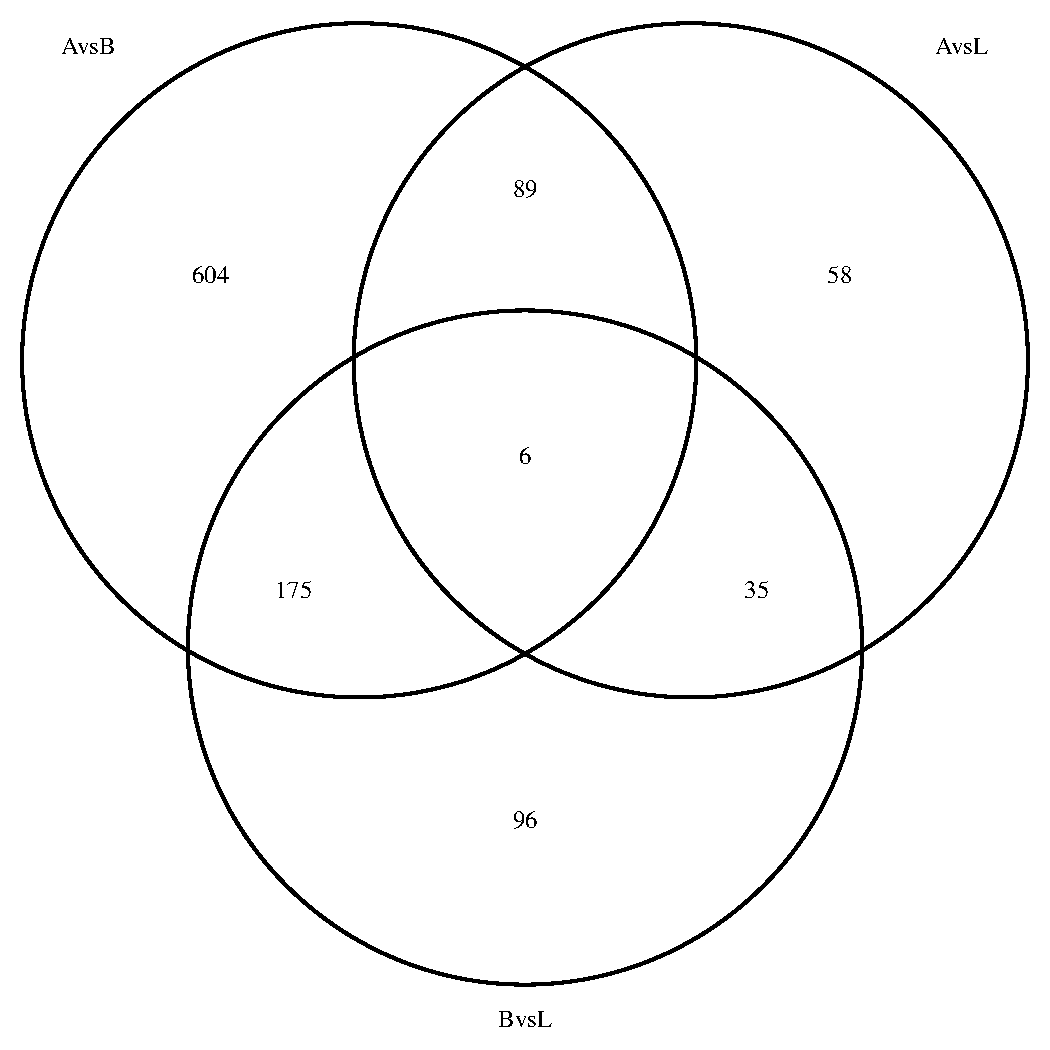
\includegraphics[width=\maxwidth]{images/graficvennSigGenes2-1} 
\begin{kframe}\begin{alltt}
\hlkwd{dev.off}\hlstd{()}
\end{alltt}
\begin{verbatim}
## null device 
##           1
\end{verbatim}
\end{kframe}
\end{knitrout}

\section{Case study}

Imagine a user wants to do the following analysis:

\begin{enumerate}
\item Select three lists from my study (\textbf{In this example we choose AvsB, AvsL, BvsL})
We can do a preliminar optional filtering to keep only genes with Entrez Identifier and remove duplicates keeping only the most variable one.
\begin{knitrout}
\definecolor{shadecolor}{rgb}{0.969, 0.969, 0.969}\color{fgcolor}\begin{kframe}
\begin{alltt}
\hlstd{AvsB0}  \hlkwb{<-} \hlkwd{genesFromTopTable} \hlstd{(AvsB,} \hlkwc{entrezOnly} \hlstd{=} \hlnum{TRUE}\hlstd{,} \hlkwc{uniqueIds}\hlstd{=}\hlnum{TRUE}\hlstd{,} \hlkwc{adjOrrawP} \hlstd{=} \hlstr{"adj"}\hlstd{,} \hlkwc{Pcutoff} \hlstd{=} \hlnum{1}\hlstd{)}
\hlstd{AvsL0}  \hlkwb{<-} \hlkwd{genesFromTopTable} \hlstd{(AvsL,} \hlkwc{entrezOnly} \hlstd{=} \hlnum{TRUE}\hlstd{,} \hlkwc{uniqueIds}\hlstd{=}\hlnum{TRUE}\hlstd{,} \hlkwc{adjOrrawP} \hlstd{=} \hlstr{"adj"}\hlstd{,} \hlkwc{Pcutoff} \hlstd{=} \hlnum{1}\hlstd{)}
\hlstd{BvsL0}  \hlkwb{<-} \hlkwd{genesFromTopTable} \hlstd{(BvsL,} \hlkwc{entrezOnly} \hlstd{=} \hlnum{TRUE}\hlstd{,} \hlkwc{uniqueIds}\hlstd{=}\hlnum{TRUE}\hlstd{,} \hlkwc{adjOrrawP} \hlstd{=} \hlstr{"adj"}\hlstd{,} \hlkwc{Pcutoff} \hlstd{=} \hlnum{1}\hlstd{)}
\end{alltt}
\end{kframe}
\end{knitrout}

\item Filter lists with adjusted-p-value less than 0.05

\begin{knitrout}
\definecolor{shadecolor}{rgb}{0.969, 0.969, 0.969}\color{fgcolor}\begin{kframe}
\begin{alltt}
\hlstd{AvsB1}  \hlkwb{<-} \hlkwd{genesFromTopTable} \hlstd{(AvsB,} \hlkwc{entrezOnly} \hlstd{=} \hlnum{TRUE}\hlstd{,} \hlkwc{uniqueIds}\hlstd{=}\hlnum{TRUE}\hlstd{,} \hlkwc{adjOrrawP} \hlstd{=} \hlstr{"adj"}\hlstd{,} \hlkwc{Pcutoff} \hlstd{=} \hlnum{0.05}\hlstd{)}
\hlstd{AvsL1}  \hlkwb{<-} \hlkwd{genesFromTopTable} \hlstd{(AvsL,} \hlkwc{entrezOnly} \hlstd{=} \hlnum{TRUE}\hlstd{,} \hlkwc{uniqueIds}\hlstd{=}\hlnum{TRUE}\hlstd{,} \hlkwc{adjOrrawP} \hlstd{=} \hlstr{"adj"}\hlstd{,} \hlkwc{Pcutoff} \hlstd{=} \hlnum{0.05}\hlstd{)}
\hlstd{BvsL1}  \hlkwb{<-} \hlkwd{genesFromTopTable} \hlstd{(BvsL,} \hlkwc{entrezOnly} \hlstd{=} \hlnum{TRUE}\hlstd{,} \hlkwc{uniqueIds}\hlstd{=}\hlnum{TRUE}\hlstd{,} \hlkwc{adjOrrawP} \hlstd{=} \hlstr{"adj"}\hlstd{,} \hlkwc{Pcutoff} \hlstd{=} \hlnum{0.05}\hlstd{)}

\hlkwd{cat}\hlstd{(}\hlstr{"AvsB: "}\hlstd{,} \hlkwd{length}\hlstd{(AvsB0),} \hlstr{"-->"}\hlstd{,} \hlkwd{length}\hlstd{(AvsB1),} \hlstr{"\textbackslash{}n"}\hlstd{)}
\end{alltt}
\begin{verbatim}
## AvsB:  708 --> 434
\end{verbatim}
\begin{alltt}
\hlkwd{cat}\hlstd{(}\hlstr{"AvsL: "}\hlstd{,} \hlkwd{length}\hlstd{(AvsL0),} \hlstr{"-->"}\hlstd{,} \hlkwd{length}\hlstd{(AvsL1),} \hlstr{"\textbackslash{}n"}\hlstd{)}
\end{alltt}
\begin{verbatim}
## AvsL:  336 --> 80
\end{verbatim}
\begin{alltt}
\hlkwd{cat}\hlstd{(}\hlstr{"BvsL: "}\hlstd{,} \hlkwd{length}\hlstd{(BvsL0),} \hlstr{"-->"}\hlstd{,} \hlkwd{length}\hlstd{(BvsL1),} \hlstr{"\textbackslash{}n"}\hlstd{)}
\end{alltt}
\begin{verbatim}
## BvsL:  412 --> 132
\end{verbatim}
\end{kframe}
\end{knitrout}

\item Create separate lists with up and down regulated genes

\begin{knitrout}
\definecolor{shadecolor}{rgb}{0.969, 0.969, 0.969}\color{fgcolor}\begin{kframe}
\begin{alltt}
\hlstd{AvsB1Up}  \hlkwb{<-} \hlkwd{genesFromTopTable} \hlstd{(AvsB,} \hlkwc{entrezOnly} \hlstd{=} \hlnum{TRUE}\hlstd{,} \hlkwc{uniqueIds}\hlstd{=}\hlnum{TRUE}\hlstd{,} \hlkwc{adjOrrawP} \hlstd{=} \hlstr{"adj"}\hlstd{,} \hlkwc{Pcutoff} \hlstd{=} \hlnum{0.05}\hlstd{,} \hlkwc{updown}\hlstd{=}\hlstr{"up"}\hlstd{)}
\hlstd{AvsL1Up}  \hlkwb{<-} \hlkwd{genesFromTopTable} \hlstd{(AvsL,} \hlkwc{entrezOnly} \hlstd{=} \hlnum{TRUE}\hlstd{,} \hlkwc{uniqueIds}\hlstd{=}\hlnum{TRUE}\hlstd{,} \hlkwc{adjOrrawP} \hlstd{=} \hlstr{"adj"}\hlstd{,} \hlkwc{Pcutoff} \hlstd{=} \hlnum{0.05}\hlstd{,} \hlkwc{updown}\hlstd{=}\hlstr{"up"}\hlstd{)}
\hlstd{BvsL1Up}  \hlkwb{<-} \hlkwd{genesFromTopTable} \hlstd{(BvsL,} \hlkwc{entrezOnly} \hlstd{=} \hlnum{TRUE}\hlstd{,} \hlkwc{uniqueIds}\hlstd{=}\hlnum{TRUE}\hlstd{,} \hlkwc{adjOrrawP} \hlstd{=} \hlstr{"adj"}\hlstd{,} \hlkwc{Pcutoff} \hlstd{=} \hlnum{0.05}\hlstd{,} \hlkwc{updown}\hlstd{=}\hlstr{"up"}\hlstd{)}
\hlkwd{cat}\hlstd{(}\hlstr{"AvsB: "}\hlstd{,} \hlkwd{length}\hlstd{(AvsB1),} \hlstr{"-->"}\hlstd{,} \hlkwd{length}\hlstd{(AvsB1Up),} \hlstr{"\textbackslash{}n"}\hlstd{)}
\end{alltt}
\begin{verbatim}
## AvsB:  434 --> 243
\end{verbatim}
\begin{alltt}
\hlkwd{cat}\hlstd{(}\hlstr{"AvsL: "}\hlstd{,} \hlkwd{length}\hlstd{(AvsL1),} \hlstr{"-->"}\hlstd{,} \hlkwd{length}\hlstd{(AvsL1Up),} \hlstr{"\textbackslash{}n"}\hlstd{)}
\end{alltt}
\begin{verbatim}
## AvsL:  80 --> 44
\end{verbatim}
\begin{alltt}
\hlkwd{cat}\hlstd{(}\hlstr{"BvsL: "}\hlstd{,} \hlkwd{length}\hlstd{(BvsL1),} \hlstr{"-->"}\hlstd{,} \hlkwd{length}\hlstd{(BvsL1Up),} \hlstr{"\textbackslash{}n"}\hlstd{)}
\end{alltt}
\begin{verbatim}
## BvsL:  132 --> 77
\end{verbatim}
\begin{alltt}
\hlstd{AvsB1Down}  \hlkwb{<-} \hlkwd{genesFromTopTable} \hlstd{(AvsB,} \hlkwc{entrezOnly} \hlstd{=} \hlnum{TRUE}\hlstd{,} \hlkwc{uniqueIds}\hlstd{=}\hlnum{TRUE}\hlstd{,} \hlkwc{adjOrrawP} \hlstd{=} \hlstr{"adj"}\hlstd{,} \hlkwc{Pcutoff} \hlstd{=} \hlnum{0.05}\hlstd{,} \hlkwc{updown}\hlstd{=}\hlstr{"down"}\hlstd{)}
\hlstd{AvsL1Down}  \hlkwb{<-} \hlkwd{genesFromTopTable} \hlstd{(AvsL,} \hlkwc{entrezOnly} \hlstd{=} \hlnum{TRUE}\hlstd{,} \hlkwc{uniqueIds}\hlstd{=}\hlnum{TRUE}\hlstd{,} \hlkwc{adjOrrawP} \hlstd{=} \hlstr{"adj"}\hlstd{,} \hlkwc{Pcutoff} \hlstd{=} \hlnum{0.05}\hlstd{,} \hlkwc{updown}\hlstd{=}\hlstr{"down"}\hlstd{)}
\hlstd{BvsL1Down}  \hlkwb{<-} \hlkwd{genesFromTopTable} \hlstd{(BvsL,} \hlkwc{entrezOnly} \hlstd{=} \hlnum{TRUE}\hlstd{,} \hlkwc{uniqueIds}\hlstd{=}\hlnum{TRUE}\hlstd{,} \hlkwc{adjOrrawP} \hlstd{=} \hlstr{"adj"}\hlstd{,} \hlkwc{Pcutoff} \hlstd{=} \hlnum{0.05}\hlstd{,} \hlkwc{updown}\hlstd{=}\hlstr{"down"}\hlstd{)}
\hlkwd{cat}\hlstd{(}\hlstr{"AvsB: "}\hlstd{,} \hlkwd{length}\hlstd{(AvsB1),} \hlstr{"-->"}\hlstd{,} \hlkwd{length}\hlstd{(AvsB1Down),} \hlstr{"\textbackslash{}n"}\hlstd{)}
\end{alltt}
\begin{verbatim}
## AvsB:  434 --> 191
\end{verbatim}
\begin{alltt}
\hlkwd{cat}\hlstd{(}\hlstr{"AvsL: "}\hlstd{,} \hlkwd{length}\hlstd{(AvsL1),} \hlstr{"-->"}\hlstd{,} \hlkwd{length}\hlstd{(AvsL1Down),} \hlstr{"\textbackslash{}n"}\hlstd{)}
\end{alltt}
\begin{verbatim}
## AvsL:  80 --> 36
\end{verbatim}
\begin{alltt}
\hlkwd{cat}\hlstd{(}\hlstr{"BvsL: "}\hlstd{,} \hlkwd{length}\hlstd{(BvsL1),} \hlstr{"-->"}\hlstd{,} \hlkwd{length}\hlstd{(BvsL1Down),} \hlstr{"\textbackslash{}n"}\hlstd{)}
\end{alltt}
\begin{verbatim}
## BvsL:  132 --> 55
\end{verbatim}
\end{kframe}
\end{knitrout}
\item Create a gene list with genes shared by AvsL and BvsL
\begin{knitrout}
\definecolor{shadecolor}{rgb}{0.969, 0.969, 0.969}\color{fgcolor}\begin{kframe}
\begin{alltt}
\hlstd{commonAvsLandBvsL} \hlkwb{<-} \hlkwd{intersect}\hlstd{(AvsL0, BvsL0)}
\hlkwd{length}\hlstd{(commonAvsLandBvsL)}
\end{alltt}
\begin{verbatim}
## [1] 104
\end{verbatim}
\end{kframe}
\end{knitrout}

\item The lists can be used from memory or written into files:

\begin{knitrout}
\definecolor{shadecolor}{rgb}{0.969, 0.969, 0.969}\color{fgcolor}\begin{kframe}
\begin{alltt}
\hlkwd{write.table}\hlstd{(}\hlkwc{x}\hlstd{=AvsB1Up,} \hlkwc{file} \hlstd{=} \hlkwd{file.path}\hlstd{(resultsDir,} \hlstr{"AvsB1Up.txt"}\hlstd{),} \hlkwc{row.names}\hlstd{=}\hlnum{FALSE}\hlstd{,} \hlkwc{col.names}\hlstd{=}\hlnum{FALSE}\hlstd{,} \hlkwc{quote}\hlstd{=}\hlnum{FALSE}\hlstd{)}
\hlkwd{write.table}\hlstd{(}\hlkwc{x}\hlstd{=AvsL1Up,} \hlkwc{file} \hlstd{=} \hlkwd{file.path}\hlstd{(resultsDir,} \hlstr{"AvsL1Up.txt"}\hlstd{),} \hlkwc{row.names}\hlstd{=}\hlnum{FALSE}\hlstd{,} \hlkwc{col.names}\hlstd{=}\hlnum{FALSE}\hlstd{,} \hlkwc{quote}\hlstd{=}\hlnum{FALSE}\hlstd{)}
\hlkwd{write.table}\hlstd{(}\hlkwc{x}\hlstd{=BvsL1Up,} \hlkwc{file} \hlstd{=} \hlkwd{file.path}\hlstd{(resultsDir,} \hlstr{"BvsL1Up.txt"}\hlstd{),} \hlkwc{row.names}\hlstd{=}\hlnum{FALSE}\hlstd{,} \hlkwc{col.names}\hlstd{=}\hlnum{FALSE}\hlstd{,} \hlkwc{quote}\hlstd{=}\hlnum{FALSE}\hlstd{)}
\hlkwd{write.table}\hlstd{(}\hlkwc{x}\hlstd{=AvsB1Down,} \hlkwc{file} \hlstd{=} \hlkwd{file.path}\hlstd{(resultsDir,} \hlstr{"AvsB1Down.txt"}\hlstd{),} \hlkwc{row.names}\hlstd{=}\hlnum{FALSE}\hlstd{,} \hlkwc{col.names}\hlstd{=}\hlnum{FALSE}\hlstd{,} \hlkwc{quote}\hlstd{=}\hlnum{FALSE}\hlstd{)}
\hlkwd{write.table}\hlstd{(}\hlkwc{x}\hlstd{=AvsL1Down,} \hlkwc{file} \hlstd{=} \hlkwd{file.path}\hlstd{(resultsDir,} \hlstr{"AvsL1Down.txt"}\hlstd{),} \hlkwc{row.names}\hlstd{=}\hlnum{FALSE}\hlstd{,} \hlkwc{col.names}\hlstd{=}\hlnum{FALSE}\hlstd{,} \hlkwc{quote}\hlstd{=}\hlnum{FALSE}\hlstd{)}
\hlkwd{write.table}\hlstd{(}\hlkwc{x}\hlstd{=BvsL1Down,} \hlkwc{file} \hlstd{=} \hlkwd{file.path}\hlstd{(resultsDir,} \hlstr{"BvsL1Down.txt"}\hlstd{),} \hlkwc{row.names}\hlstd{=}\hlnum{FALSE}\hlstd{,} \hlkwc{col.names}\hlstd{=}\hlnum{FALSE}\hlstd{,} \hlkwc{quote}\hlstd{=}\hlnum{FALSE}\hlstd{)}
\hlkwd{write.table}\hlstd{(}\hlkwc{x}\hlstd{=commonAvsLandBvsL,} \hlkwc{file} \hlstd{=} \hlkwd{file.path}\hlstd{(resultsDir,} \hlstr{"commonAvsLandBvsL.txt"}\hlstd{),} \hlkwc{row.names}\hlstd{=}\hlnum{FALSE}\hlstd{,} \hlkwc{col.names}\hlstd{=}\hlnum{FALSE}\hlstd{,} \hlkwc{quote}\hlstd{=}\hlnum{FALSE}\hlstd{)}
\end{alltt}
\end{kframe}
\end{knitrout}



\end{enumerate}

\bibliography{MDAreferences}

\end{document}

%%%%%%%%%%%%%%%%%%% Old code




